\documentclass[12pt]{article}
\usepackage{graphicx}
\usepackage{hyperref}
\usepackage{subcaption}
\usepackage{amsmath}
\usepackage{geometry}
\usepackage{float} % Include the float package
\geometry{a4paper}

\title{Comprehensive Analysis Report of the WhatsApp Group: Pakistan Monji}
\author{Muhammad Saad}
\date{\today}

\begin{document}

\maketitle

\section{Introduction}
This document presents a detailed analysis of the WhatsApp group "Pakistan Monji," which focuses on agricultural discussions, particularly related to rice. The analysis delves into various types of interactions within the group, including the sharing of media, textual communications, and promotional activities. By examining these elements, this report aims to highlight the dynamics of communication, the relevance of shared content to the group's goals, and the engagement levels of its members.


\section{Data Analysis}
\subsection{Irrelevant Marketing Posts}
Despite the group's focus on agricultural information and discussions about rice, there are several messages that can be identified as marketing posts that do not align with the group’s main objective. Below are examples of such marketing posts identified in the provided text:

\begin{itemize}
\item \textbf{Message 7:} Promotes a special offer during Bari Eid, which, while loosely related to community celebrations, primarily serves as a sales tactic.
\item \textbf{Message 22:} Endorses SadaPay, a financial service unrelated to agriculture, highlighting a misalignment with the group's intended content.
\item \textbf{Message 39:} Announces an ``End Season Sale," which, despite its potential relevance to agricultural product clearing, primarily functions as a commercial sales pitch.
\end{itemize}



\subsection{Group Invitations}
The group contains only 1 invite link to a WhatsApp group called ``Asia best rice and paddy corn group". This shows similar other groups are being promoted in the group.
\begin{figure}[H]
\centering
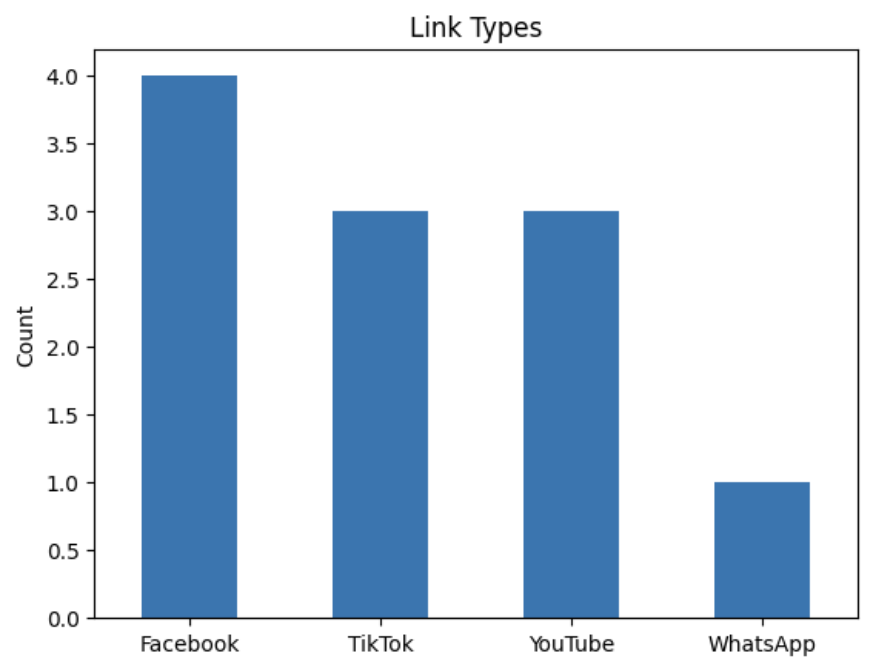
\includegraphics[width=0.8\textwidth]{img/group_invitations.png}
\caption{Group Invitations Analysis}
\end{figure}

\subsection{Response Posts}
Users do not usually interact with the other posts in the group. Replies are usually done if the user missed something in the earlier message.  \textbf{Likes} and \textbf{emojis} are the most common form of response. In general, the group does not contain any interactive discussions.



\subsection{Useful Content \& Irrelevant Content}
Detailed analysis is provided in section 3.1.

\section{Medium Analysis}
\subsection{Text Messages}

\subsubsection{Religious Messages}
These messages contain spiritual sentiments, religious teachings, or prayers, unrelated to agricultural discussions.
\begin{itemize}
  \item \textbf{Message 11:} Discusses divine justice and historical religious events related to the incident of camel's leg being cut.
  \item \textbf{Message 12:} A prayer for divine retribution against an oppressor.
  \item \textbf{Message 13-15:} Various prayers and religious affirmations.
  \item \textbf{Message 17:} Describes Prophet's sermon, its content and implications.
  \item \textbf{Message 35:} Reflects on historical religious events and their moral lessons.
\end{itemize}

\subsubsection{Political Messages}
These involve mentions of political or historical contexts that are not directly related to agriculture.
\begin{itemize}
  \item \textbf{Message 40:} Implicit criticism of judicial inaction, potentially political in nature.
\end{itemize}

\subsubsection{Useful Messages (Agriculture and Rice)}
These messages directly contribute to the group's primary focus on sharing valuable agricultural information, particularly related to rice cultivation and related agricultural issues. Examples include:
\begin{itemize}
  \item \textbf{Rice Varieties (Message 3 \& 4)}: Discusses successful rice varieties and provides names like 1847 Anarkali and 1509, which are likely types of rice, contributing to knowledge about different cultivars suitable for local farming conditions.
  \item \textbf{Sales Tax Inquiry (Message 20)}: Asks about sales tax implications on rice exports, indicating a concern for the economic aspects of rice farming and trade, vital for members involved in the commercial side of agriculture.
  \item \textbf{Bulk Corn Transaction (Message 28)}: Involves a request for a significant amount of corn, showing trade and logistics within the group, which can be crucial for farmers looking to buy or sell in bulk.
  \item \textbf{Price Inquiries (Messages 29-31)}: These messages asking for rates likely relate to agricultural products, demonstrating active market participation by group members.
  \item \textbf{Rice Availability (Message 36)}: Seeks information on the availability of Iri 6 rice in various regions, pertinent for those looking to purchase or sell this staple crop.
\end{itemize}


\subsection{Photos \& Videos}
\begin{itemize}
  \item \textbf{Religious and Cultural Celebrations}: Images and graphics celebrating Islamic holidays such as Eid, adorned with religious calligraphy and symbols, fostering spiritual connections and communal solidarity.
  \item \textbf{Government and Official Announcements}: Official press releases and updates, such as those detailing changes in petroleum prices by the Government of Pakistan, providing members with crucial national economic information.
  \item \textbf{Marketing and Promotions}: Promotional images advertising products like herbal remedies or agricultural items, aimed at supporting local businesses or relevant products for the group's members.
  \item \textbf{Health and Medical Issues}: Photos depicting medical conditions, possibly to raise awareness, offer advice, or mobilize support for health-related issues within the community.
\end{itemize}

\subsection{Voice Notes}
The group contains only 2 voice notes. The first one wishes Eid in punjabi. Very hard to understand again. The second voice note is a very calm person defending a culinary place as someone had found a fly in one of their dishes. Its in Urdu so easy to understand.

\section{User Insights}
\subsection{Number of Admins}
There is only 1 admin in the group.

\subsection{Total Users}
The total number of users in the group is 577.

\subsection{Active Users}
There are 26 active users, who regularly contribute to the discussions. Top 20 are:
\begin{enumerate}
  \item Muhammad Jawed
  \item Aziz
  \item +92 300 0265758
  \item Ikhlaq Ahmad Mahni Sial
  \item +93 78 939 3463
  \item Naveed Ahmad
  \item saadullah0945
  \item Rana Hameed Zaildar
  \item khawarrafique709
  \item alimafadshahshah
  \item Hafiz Jazim Noori
  \item +92 300 7888284
  \item zulqarnainhundal
  \item +92 320 1749211
  \item mw705167
  \item Ramzan Gujjar
  \item Malik Sabir
  \item +92 300 3484784
  \item Ch
  \item Irfan Bhutta
\end{enumerate}
\begin{figure}[H]
  \centering
  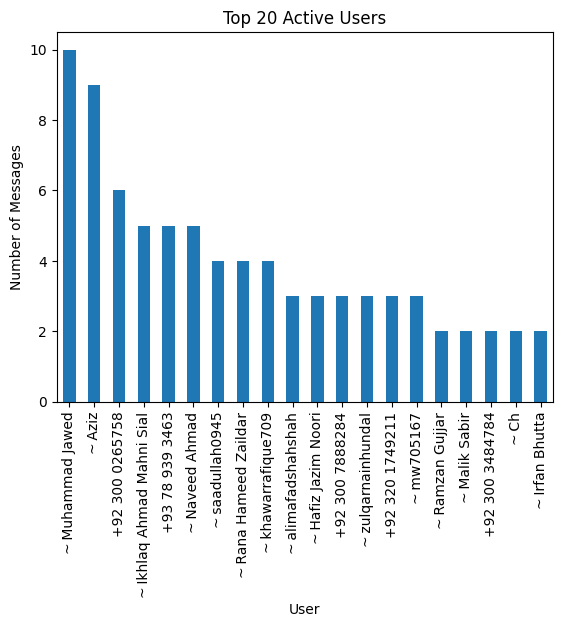
\includegraphics[width=0.8\textwidth]{img/active_users.png}
  \caption{Top 20 Active Users by messages}
\end{figure}

\section{Main Talking Points}
The main talking points in the group are:
\begin{itemize}
  \item Agricultural Practices and Techniques
  \item Commercial Transactions and Market Information
  \item Economic Aspects Related to Agriculture
\end{itemize}

\section{Time of Posting}
The most active posting times are 7-9 AM, 12-4 PM and 9 PM, as shown in the chart below.
\begin{figure}[H]
\centering
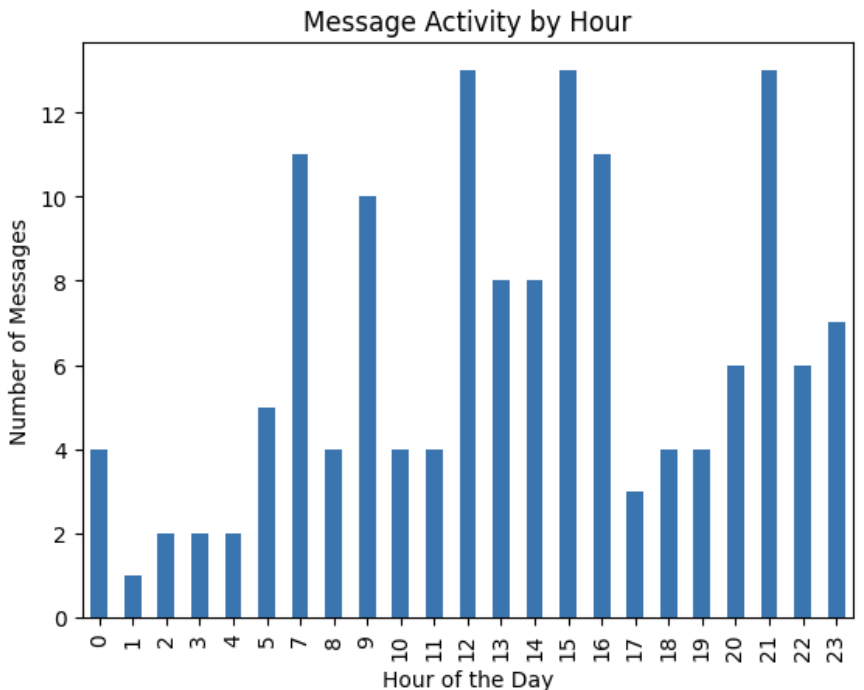
\includegraphics[width=0.8\textwidth]{img/posting_times.png}
\caption{Message Activity by Hour}
\end{figure}

\section{Preferred Medium of Posting}
Text, photos, and videos are the most preferred mediums for posting in the group, as shown in the chart below.
\begin{figure}[H]
\centering
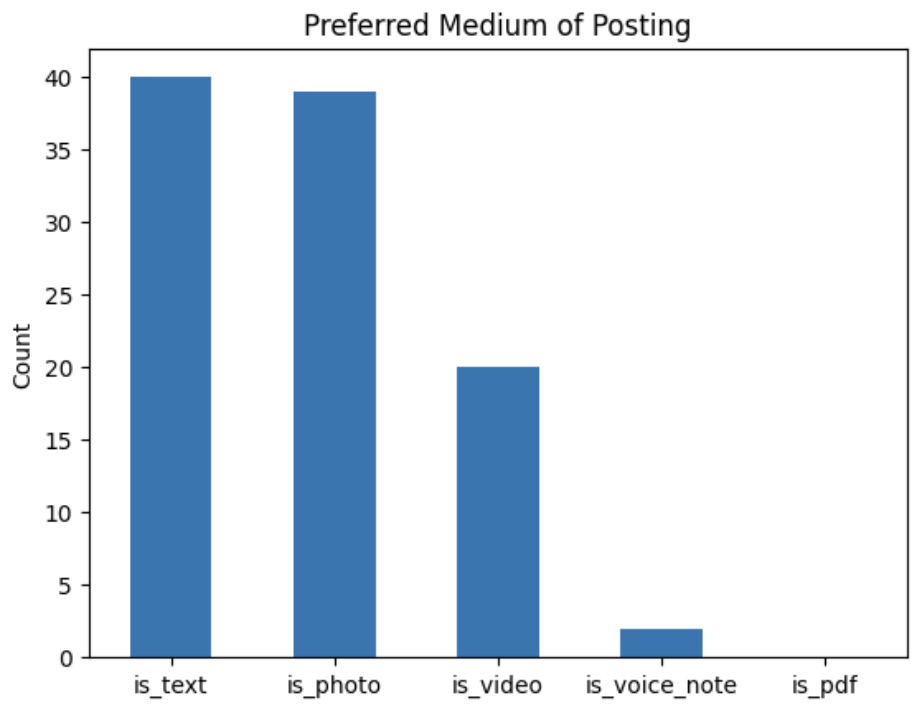
\includegraphics[width=0.8\textwidth]{img/medium_preference.png}
\caption{Preferred Mediums of Posting}
\end{figure}

\section{Conclusion}
The comprehensive analysis of the "Pakistan Monji" WhatsApp group reveals a vibrant community engaged in diverse discussions that span agricultural practices, religious celebrations, and economic updates. While the group serves as a critical resource for agricultural information and local market updates, it also encapsulates a cultural and communal hub for its members.

\end{document}
